%%%%%%%%%%%%%%%%%%%%%%%%%%%%%%%%%%%%%%%%%%%%%%%%%%%%%%%%%%%%%%%%%%%%%%%%
% Plantilla TFG/TFM
% Escuela Politécnica Superior de la Universidad de Alicante
% Realizado por: Jose Manuel Requena Plens
% Contacto: info@jmrplens.com / Telegram:@jmrplens
%%%%%%%%%%%%%%%%%%%%%%%%%%%%%%%%%%%%%%%%%%%%%%%%%%%%%%%%%%%%%%%%%%%%%%%%

\chapter{Estado del Arte}

En este capítulo se presentan las principales soluciones existentes en el ámbito de la monitorización de redes. El objetivo es identificar sus características más relevantes, así como sus ventajas y limitaciones, de manera que sirvan como referencia para el diseño del sistema propuesto en este trabajo.

\section{Nagios: Sistema de Monitorización de Redes}
Nagios es una de las soluciones más utilizadas en el ámbito de la monitorización de infraestructuras IT. Su capacidad de supervisar redes, servidores y aplicaciones la convierten en una opción versátil y ampliamente adoptada en entornos empresariales. 

Uno de los principales productos de Nagios es Nagios XI, el cual proporciona un conjunto de herramientas avanzadas para la monitorización de infraestructuras críticas \citep{nagios2014}. Este software perminte supervisar el estado de aplicaciones, servicios, sistemas operativos y protocolos de red. Además, cuenta con un sistema de alertas en tiempo real que notifica a los administradores mediante correo electrónico, SMS o mensajería instantánea. Tiene la capacidad de generar informes detallados sobre el historial de fallos, análisis de tendencias y planificación de capacidad es otra de sus características más destacadas. Una de las fortalezas es su interfaz web, la cual permite a los usuarios personalizar paneles de control para visualizar métricas clave \citep{nagios2014}.

\begin{figure}[H]
    \centering
    {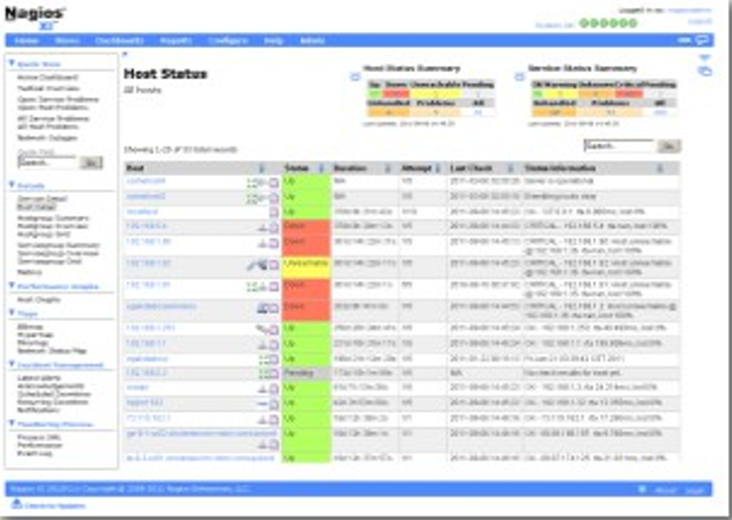
\includegraphics[width=0.7\linewidth]{imagenes/image2.png}}
    \caption{Ejemplo visual de Nagios XI \citep{nagios2014}}
    \label{fig:enter-label}
\end{figure}

Otro componente relevante es Nagio Fusion, diseñado para proporcionar una vista consolidad de múltiples instancias de Nagios \citep{nagios2014}. A gran escala, esta herramienta resulta especialmente útil, ya que permite gestionar diferentes servidores de monitoreo desde una única plataforma \citep{nagios2014}.

\begin{figure}[H]
    \centering
    {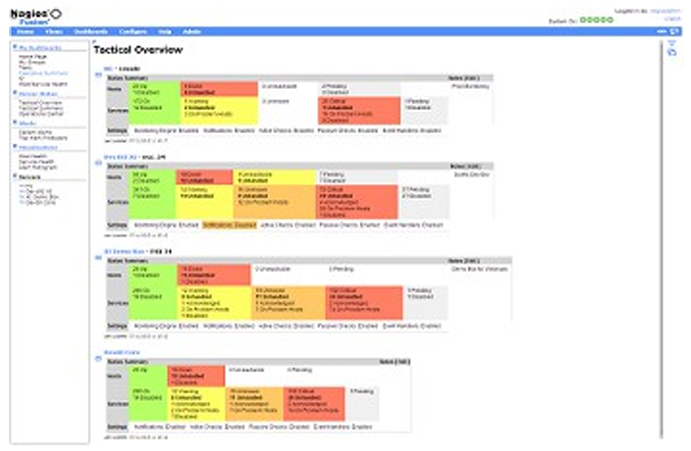
\includegraphics[width=0.7\linewidth]{imagenes/image3.png}}
    \caption{Ejemplo visual de Nagios Fusion \citep{nagios2014}.}
    \label{fig:enter-label}
\end{figure}

En el ámbito de la gestión de incidentes, Nagios Incident Manager facilita  la administración de alertas y eventos críticos detectados por Nagios XI \citep{nagios2014}. Su integración permite la creación y la asignación de tickets en tiempo real, fomentando la colaboración entre equipos IT y agilizando la resolución de problemas.

\begin{figure}[H]
    \centering
    {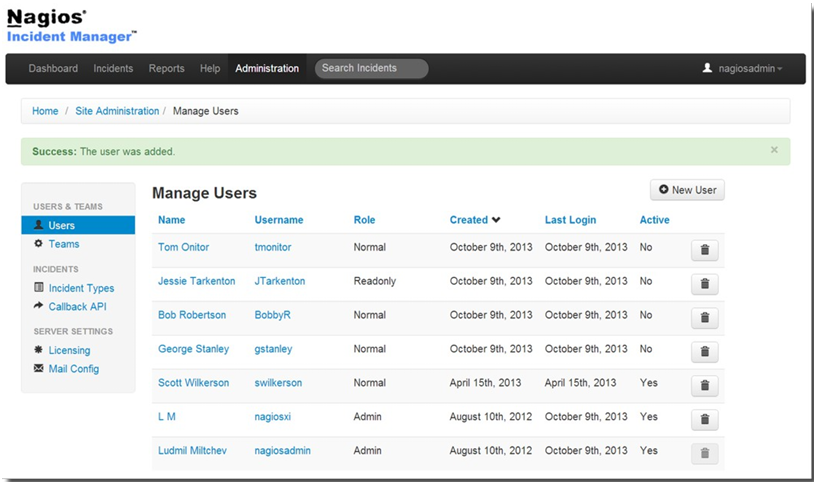
\includegraphics[width=0.7\linewidth]{imagenes/image4.png}}
    \caption{Ejemplo visual de Nagios Incident Manager \citep{nagios2014}.}
    \label{fig:enter-label}
\end{figure}

Por otro lado, Nagios Network Analyzer se enfoca en el análisis de tráfico de red \citep{nagios2014}. Esta herramienta permite supervisar el uso del ancho de banda y detectar patrones de tráfico que pueden indicar problemas o posibles amenazas de seguridad. Su compatibilidad con tecnologías como NetFlow y sFlow permite recopilar información detallada sobre el tráfico en la red, alertando a los administradores en caso de picos inusuales o comportamientos anómalos. Además, su capacidad de generar gráficos avanzados facilita la interpretación de datos y el diagnóstico de problemas en la red \citep{nagios2014}.

\begin{figure}[H]
    \centering
    {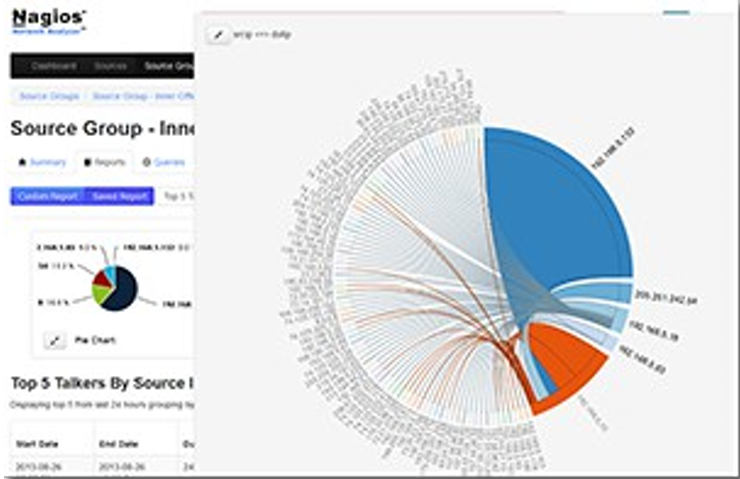
\includegraphics[width=0.7\linewidth]{imagenes/image5.png}}
    \caption{Ejemplo Visual de Nagios Network Analyzer \citep{nagios2014}.}
    \label{fig:enter-label}
\end{figure}

Dentro del contexto del Trabajo final de Máster, Nagios representa un modelo robusto que puede servir de referencia. En particular, Nagios XI y Nagios Network Analyzer, la posibilidad de personalizar dashboards, gestionar alertas en tiempo real y analizar tráfico de red son clave en la planificación y el diseño del trabajo.

Sin embargo, también es importante indicar las limitaciones del software. Aunque su sistema de monitorización es configurable, puede requerir una curva de aprendizaje elevada, especialmente para administradores sin experiencia previa. Además, su modelo basado en plugins y extensiones puede hacer que la integración de otros sitemas requiera una configuración adicional.
% Aquí copiarías lo que ya tienes desarrollado sobre Nagios (texto + figuras).

\section{Zabbix: Sistema de Monitorización de Redes}
Zabbix es una plataforma de monitorización de código abierto que ha sido ampliamente adoptada en la industria debido a su flexibilidad, escalabilidad y capacidad de integración con diversas tecnologías.

% Aquí copiarías el bloque de Zabbix.

\section{Prometheus: Sistema de Monitorización de Redes}
Prometheus es una plataforma de monitorización y alerta de código abierto diseñada para la recolección y análisis de métricas en entornos dinámicos.

% Aquí copiarías lo de Prometheus.

\section{SolarWinds Network Performance Monitor}
SolarWinds Network Performance Monitor (NPM) es una solución comercial diseñada para proporcionar una visión integral del estado y rendimiento de infraestructuras de redes de comunicaciones.

% Aquí copias lo de SolarWinds.

\section{PRTG Network Monitor}
PRTG Network Monitor, desarrollado por Paessler AG, es una plataforma de monitorización de redes que destaca por su enfoque integral, intuitivo y escalable.

% Aquí copias lo de PRTG.

\section{Comparativa de herramientas}
Con el fin de obtener una visión global, en la Figura~\ref{fig:comparativa} se presenta una tabla comparativa que sintetiza las características principales de las herramientas analizadas.

\begin{figure}[H]
    \centering
    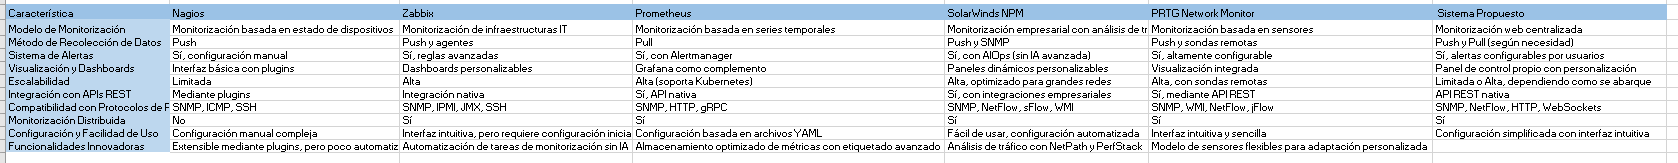
\includegraphics[width=\textwidth]{imagenes/image13.png}
    \caption{Tabla comparativa con los sistemas de monitorización analizados.}
    \label{fig:comparativa}
\end{figure}

\section{Conclusiones del estado del arte}
Del análisis realizado se desprende que:
\begin{itemize}
    \item \textbf{Nagios} y \textbf{Zabbix} son soluciones robustas y muy extendidas, aunque pueden requerir una curva de aprendizaje elevada.
    \item \textbf{Prometheus}, en combinación con Grafana, se ha consolidado como la opción preferida en entornos de microservicios y Kubernetes.
    \item \textbf{SolarWinds} y \textbf{PRTG} ofrecen soluciones comerciales completas, con interfaces gráficas avanzadas, pero requieren licencias de pago.
    \item Todas las herramientas incorporan mecanismos de alertas y notificaciones, siendo este un elemento esencial en la gestión proactiva de redes.
\end{itemize}

En conclusión, cada herramienta presenta fortalezas y debilidades, lo que evidencia la necesidad de un sistema que combine escalabilidad, facilidad de uso y capacidad de detección de anomalías. Este enfoque será el que guíe el desarrollo del presente TFM.